
\section{LAR wing Lift and Drag Models}

Low aspect ratio wings have small ratio between the wing span and
the chord. Commertial aircrafts typically have high aspect ratio wings
to increase the amount of lift on the aircraft, but there are benefits of having
low aspect wings. Low aspect ratio aircrafts need to deal with less bending
stress because the wings are shorter. Also, the drag due to surface friction is
smaller because of the lower Reynolds number from the bigger length scale.
For paper airplanes, low aspect ratio wings are definitely better than high
aspect ratio wings because paper cannot overcome the bending stress.


\subsection{Previous Research}

A lot of research about the lift and drag of wings with low aspect ratios  were done in the form of
micro-air vechicle research. This has the most relevance with paper airplanes because
micro-air vehicles operate on a Reynold number regime similar to paper airplanes. 
In 1999, Mueller showed that cambered plates offer better performance than flat plate wings, and
trailing-edge geometry does not have a strong effect on lift and drag
for thing wings at low Reynolds numbers. Also many experiments were done to experimentally
find the lift and drag coefficient of different wing shapes of different aspect ratios.

\subsection{Flat Plate model}

One way to model the wings is as a flat plane that is infinite in length. This corresonds to
an aspect ratio of zero. Since it is
an infinite flat plate, we can analyze it with a complex potential in two dimensions.
By means of conformal mapping, we can collapse a cylinder to a flat plate by

\[Z = z + \frac{a^2}{z}\].

\begin{figure}[hl]
  \centering
    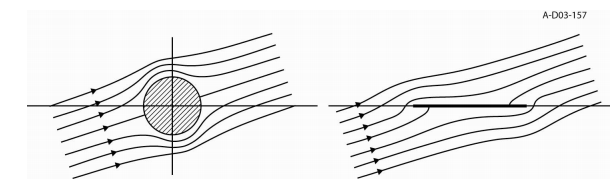
\includegraphics[scale=.5]{figures/flatplate1.png}
    \caption{An illustration of the conformal mapping from a cylinder to a flat plate. Figure adapted from ~\cite{thintheory}}
  \label{fig:dihedraleffect}
\end{figure}

Now let us consider a flow at an angle $\alpha$. A cylinder with a radius $r$
would result in a potential
\[w(z) = Ue^{i\alpha}(z + \frac{a^2}{z}) \]
After the conformal transformation, we see that the velocity now becomes
\[u - iv = \od{W}{Z} = \frac{\od{w}{z}}{\od{Z}{z}} = \frac{Ue^{-i\alpha}-Ue^{i\alpha}\frac{a^2}{z^2}
- \frac{i \Gamma}{2\pi z}}{1 - \frac{a^2}{z^2}}\]

In order to choose $\Gamma$ we must use the fact that the singularity at the trailing edge, 
$Z=2a$ or $z=a$ must be removed, from the Kutta condition. This condition occurs because 
a boundary layer prevents the flow from turning the sharp corner at the trailing edge.
The physical solution from complex flow theory depends on frictional forces.

Therefore we can find the circulation

\[ \Gamma = -4\pi Ua \sin(\alpha) \]

This allows us to find the lift by the Kutta-Joukowski theorem

\[L = \rho U \Gamma\]
\begin{equation}
\label{eq:flat_plat_cl}
C_L = 2\pi sin(\alpha)
\end{equation}

\subsection{Bollay Models}

The problem with the flat plate in the previous chapter is that it had to assume 
an aspect ratio of about zero in order to model it in that fashion. However, we can still
use the fact that the aspect ratio is small the model it in a similar fashion.
Let us assume that the wing is thin and has a low aspect ratio. Let the angle of attack
 be $\alpha$ and the velocity of the flow relative to the wing be $v$. 
 We can see that the normal component of the air
will have velocity $V\sin(\theta)$. Because the aspect ratio is low
we can model the flow around the wing like the flat plate model above.
This is depicted in Figure~\ref{fig:bollay1}

\begin{figure}[hl]
  \centering
    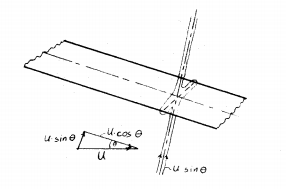
\includegraphics[scale=1]{figures/bollay1.png}
    \caption{An illustration of the flow around low aspect ratio wing. Figure adapted from~\cite{bollay}}
  \label{fig:bollay1}
\end{figure}


\[V\sin(\alpha)\]

If the angle is small enough this is approximately

\[V\alpha\]


It then follows that the lift force per unit length is just the normal velocity $V\alpha$ times the
rate of increase of a virtual additional mass. The virtual additional mass comes from the
added inertia from the fluid moving around the immersed object. From~\cite{jones} it is know that.

\begin{equation}
dm=\frac{\pi}{4}\rho b^2 dx
\end{equation}

If $\rho$ is the density of the fluid and $b$ and $x$ are the dimensions of the plate.

\[l = V\alpha \od{m}{t} = V^2\alpha \od{m}{x} \]

\[l = \pi \alpha \frac{\rho}{2}V^2 b \od{b}{x} \dif{x} \]

\[l = \pi \alpha \frac{\rho}{2} V^2 b \dif{b} \]

To get the entire lift force we can just integrate across the width of the wake. 

\[L = \frac{\pi \alpha \rho V^2 b_{max}}{4} \]

This results in a lift coefficient $C_L$ of

\begin{equation}
 \frac{\pi}{2} \AR \alpha 
 \label{eq:bollay_model}
 \end{equation}

Where $\AR$ is the aspect ratio. In the experiments section we will test whether or not the aspect ratio
would actually affect the lift coefficient.




